\documentclass[%
	corpo=11pt,
    twoside,
    stile=classica,
    oldstyle,
    tipotesi=custom,
    greek,
    evenboxes,
]{toptesi}
%%%%%%%%%%%%%%%%%%%%%%%%%%%%%%%%%%%%%%%%%%%%%%%%%%%%

\usepackage[utf8]{inputenc}
\usepackage[T1]{fontenc}
\usepackage{lmodern}

\usepackage{hyperref}
\hypersetup{%
    pdfpagemode={UseOutlines},
    bookmarksopen,
    pdfstartview={FitH},
    colorlinks,
    linkcolor={blue},
    citecolor={blue},
    urlcolor={blue}
  }

%%%%%%% use PDFLATEX 

\usepackage{stix}
\usepackage{epigraph}

\usepackage{lipsum} %to insert random text

\usepackage{geometry} %for the margins
\newcommand\fillin[1][4cm]{\makebox[#1]{\dotfill}} %for the dotted line in the frontispiace

\usepackage{dcolumn}
\newcolumntype{d}{D{.}{.}{-1} } %to vetical align numbers in tables, along the decimal dot

\usepackage{amsmath}

\usepackage{natbib} % for the bibliography
\bibliographystyle{plainnat}


%%%%%%% Local definitions
\newtheorem{osservazione}{Osservazione}% Standard LaTeX
\newtheorem{observation}{Observation}% Standard LaTeX




%%%%%%%%%%%%%%%%%%%%%%%%%%%%%%%%%%%%%%%%%%%%%%%%
%%%%%%%%%%%%%%%%%%%%%%%%%%%%%%%%%%%%%%%%%%%%%%%%



\begin{document}\errorcontextlines=9
%\english

\begin{titlepage}
\newgeometry{left=1cm,right=1cm,top=3cm,bottom=3.5cm}  %specific margins for this page

\begin{center}

{\huge POLITECNICO DI TORINO}\\[1.5cm]
\textbf{Corso di Laurea\\in Matematica per l'Ingegneria}\\[3cm]
%\textbf{Corso di Laurea Magistrale\\in Ingegneria Matematica}\\[3cm]

{\Large Tesi di Laurea}\\[1cm]
%{\Large Tesi di Laurea Magistrale}\\[0.5cm]
\textbf{\LARGE Filtraggio di immagini }\\[2cm]

\includegraphics[width=0.2\textwidth]{./Pictures/logo_polito_2021.jpg}
\vspace{4cm}


\begin{minipage}{0.85\textwidth}
\begin{flushleft}\large
\textbf{Relatori} \hfill \textbf{Candidato}\\
prof. Nome Cognome \hfill Raffaello Ippolito\\
prof. Nome Cognome \\
\textit{firma dei relatori} \hfill \textit{firma del candidato}\\[0.35cm]
\fillin\ \hfill \\
\fillin\ \hfill \fillin
\end{flushleft}
\end{minipage}

\vfill

Anno Accademico 2021-2022
\end{center}

\restoregeometry %restor default margins 

\end{titlepage} %the frontispiece

%%%%%%% Dedication
\ifclassica%
{\begin{dedica}

    $\heartsuit$\ Alla mia regina
\end{dedica}
%%%%%%% 

\sommario%summary
%Here goes the abstrat of your thesis
Lo studio delle Equazioni alle derivate parziali ed il loro impiego in ambito di filtraggio di immagini.

%%%%%%%%%%%%%%%%%%%%%%%%%%%%%%%%%%%%%%%%%%%%%%%%
%%%%%%%%%%%%%%%%%%%%%%%%%%%%%%%%%%%%%%%%%%%%%%%%

\ringraziamenti%acknowledgements
%Acknowledge the people you love and/or work with
I candidati ringraziano vivamente il Granduca di Toscana per i mezzi messi loro a disposizione, ed il signor Von Braun, assistente del prof.~Albert Einstein, per le informazioni riservate che egli ha gentilmente fornito loro, e per le utili discussioni che hanno permesso ai candidati di evitare di riscoprire l'acqua calda.

%%%%%%%%%%%%%%%%%%%%%%%%%%%%%%%%%%%%%%%%%%%%%%%%
%%%%%%%%%%%%%%%%%%%%%%%%%%%%%%%%%%%%%%%%%%%%%%%%

\tablespagetrue\figurespagetrue%to include the list of tables
%and the list of figures - yuo can comment these commands

\indici%table of content
%It automatically generated

%%%%%%%%%%%%%%%%%%%%%%%%%%%%%%%%%%%%%%%%%%%%%%%%
%%%%%%%%%%%%%%%%%%%%%%%%%%%%%%%%%%%%%%%%%%%%%%%%

%Citation
%If you feel like a poetic guy!
\ifclassica   
\begin{citazioni}
    \textit{If you cannot understand my\\argument, and declare}\\
    it's Greek to me\\
    \textit{you are quoting Shakespeare.}
    
    [\textsc{B. Levin}, Quoting Shakespeare]\vspace{1em}
\end{citazioni}
\fi

%%%%%%%%%%%%%%%%%%%%%%%%%%%%%%%%%%%%%%%%%%%%%%%%
%%%%%%%%%%%%%%%%%%%%%%%%%%%%%%%%%%%%%%%%%%%%%%%%

\mainmatter

\part{Introduzione}
\chapter{Nozioni introduttive}

\section{Introduzione}
Le immagini hanno un ruolo fondamentale nelle nostre vite, viviamo di immagini, ne guardiamo tutti i giorni in tutti i contesti, la percezione visiva è sempre il nostro primo riferimento senza la quale ci si sentiamo persi.
Viviamo in una società consapevole di ciò e che sfrutta questo aspetto quanto più possibile nei campi più disparati, fotografie, radiografie, ecografie, poster pubblicitari, progetti, etc.
E' quindi un problema sempre di grande interesse cercare di sfruttarle al meglio, a tal fine esistono metodi cosìdetti di "filtraggio", tramite i quali intendiamo migliorare la qualità delle nostre immagini, mettere in risalto determinate caratteristiche o nasconderne altre.

Viviamo in un era digitale, le immagini passano generalmente per un calcolatore prima di essere stampate, o in ogni caso possono essere sempre scannerizzate (con strumenti più o meno precisi) così da averne una copia digitale.
E' in questa fase che l'immagine subisce il processo di filtraggio, nel calcolatore, quando pè in formato digitale, Per capire cos'è un filtro occorre dunque chiedersi cosa sia un'immagine digitale.

\section{Immagini digitali}
Per capire come codificare un'immagine per memorizzarla in fgormato digitale ci chiediamo prima che cos'è un'immagine.

\begin{quote}
\epigraph{Forma esteriore degli oggetti corporei, in quanto viene percepita attraverso il senso della vista, o si riflette – come realmente è, o variamente alterata – in uno specchio, nell’acqua e sim., o rimane impressa in una lastra o pellicola o carta fotografica.}{Vocabolario Treccani}
\end{quote}


Un'immagine viene rappresentata, impressa quindi su superfici, cioè oggetti bidimensionali, di dimensioni finite e le vediamo perchè i nostri occhi percepiscono il susseguirsi di colori diversi. Come codificare tali entità?
Come tutti gli oggetti reali, sebbene abbiano dimensioni finite, il susseguirsi delle immagini avviene in una maniera che possiamo considerare come continua. Questo è il primo problema che ci si pone quando si pensa a come codificare delle immagini.
La soluzione più largamente utilizzata è anche quella più semplice ed intuitiva, ossia di discretizzare tale distribuzione di colori. Dividiamo l'immagine con una griglia ed ad ogni casella, che d'ora in poi chiameremo "pixel", assegnamo un colore. 
E' ovvio che così facendo si perdono dei dettagli, la quantità di dettagli che riusciamo a conservare piò variare enormemente, un minimo si perde sempre ma è un  prezzo che siamo disposti a pagare.


Facciamo un esempio

%\ref{fig:figuraa}. 
\begin{figure}[htb] \centering
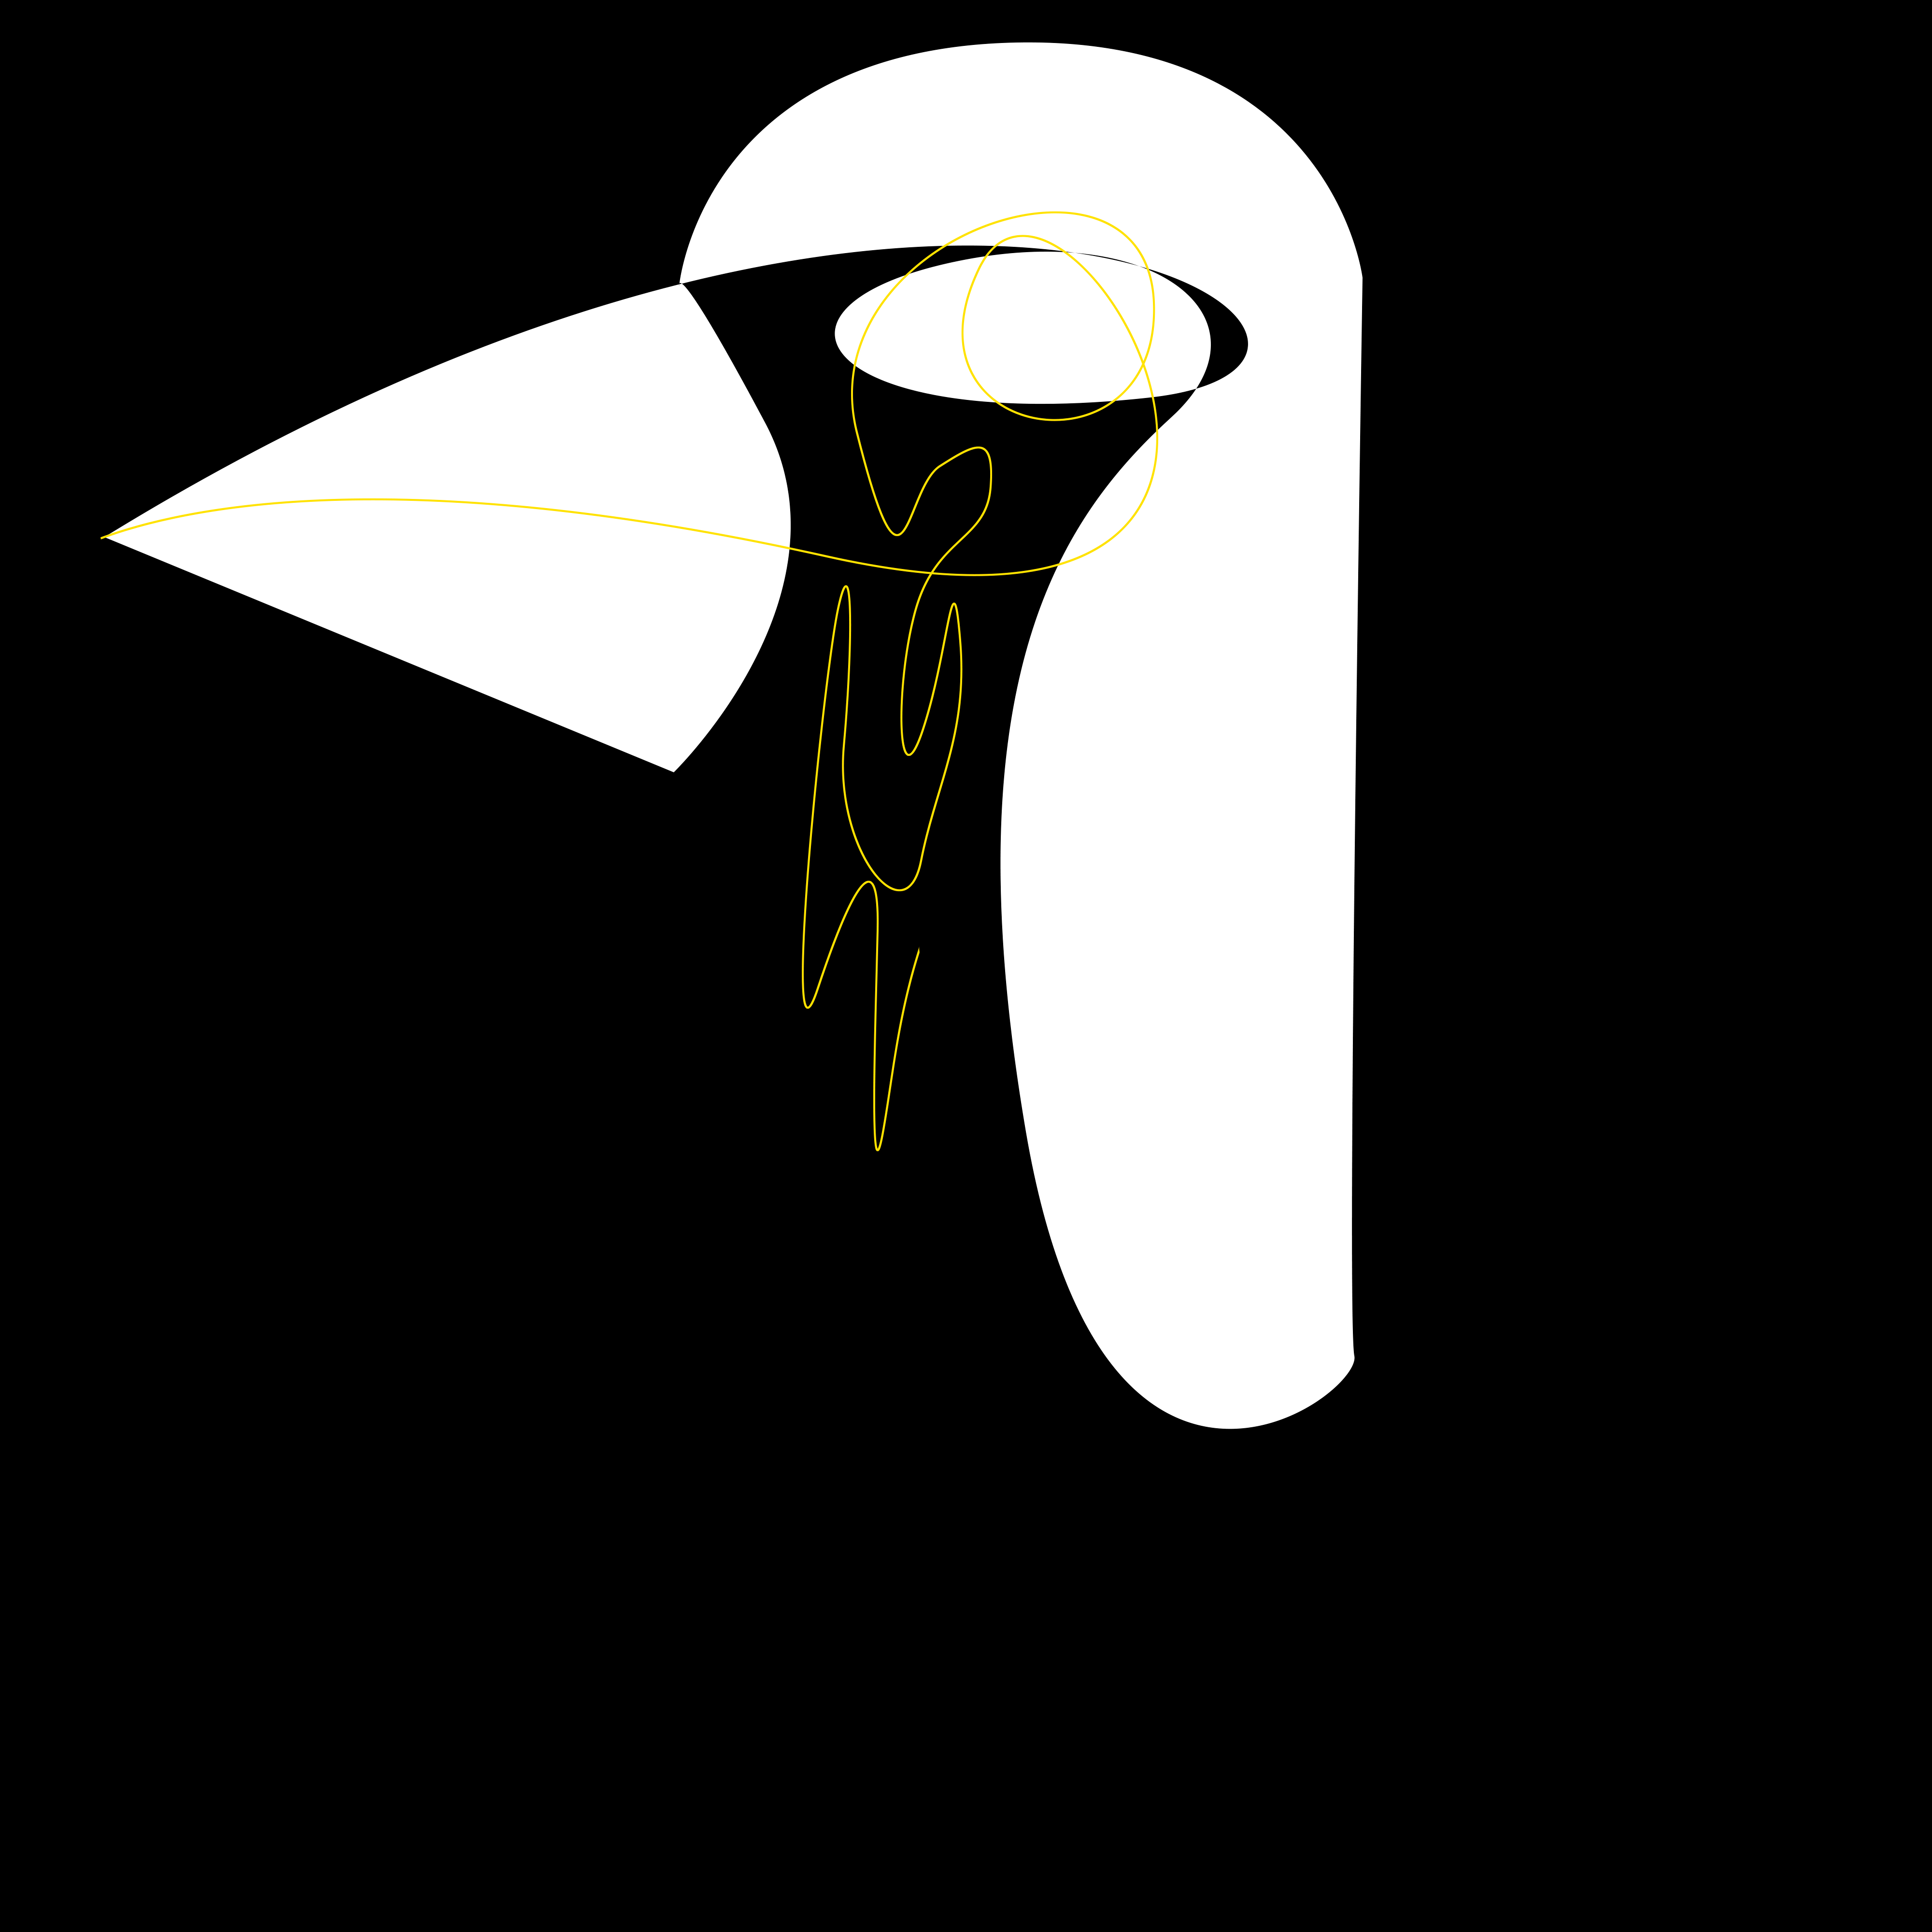
\includegraphics[scale=0.03]{Pictures/in ricordo del pinguino cameriere.png}
%\caption{Fiamme.}\label{fig:figura}
\qquad\qquad

\includegraphics[scale=0.03]{Pictures/canvas8x8.png}
\caption{Confronto immagine originale e immagine codificate utilizzando una griglia 4x4.}\label{fig:figura}
\end{figure}

%\ref{fig:figura}. 
\begin{figure}[htb] \centering
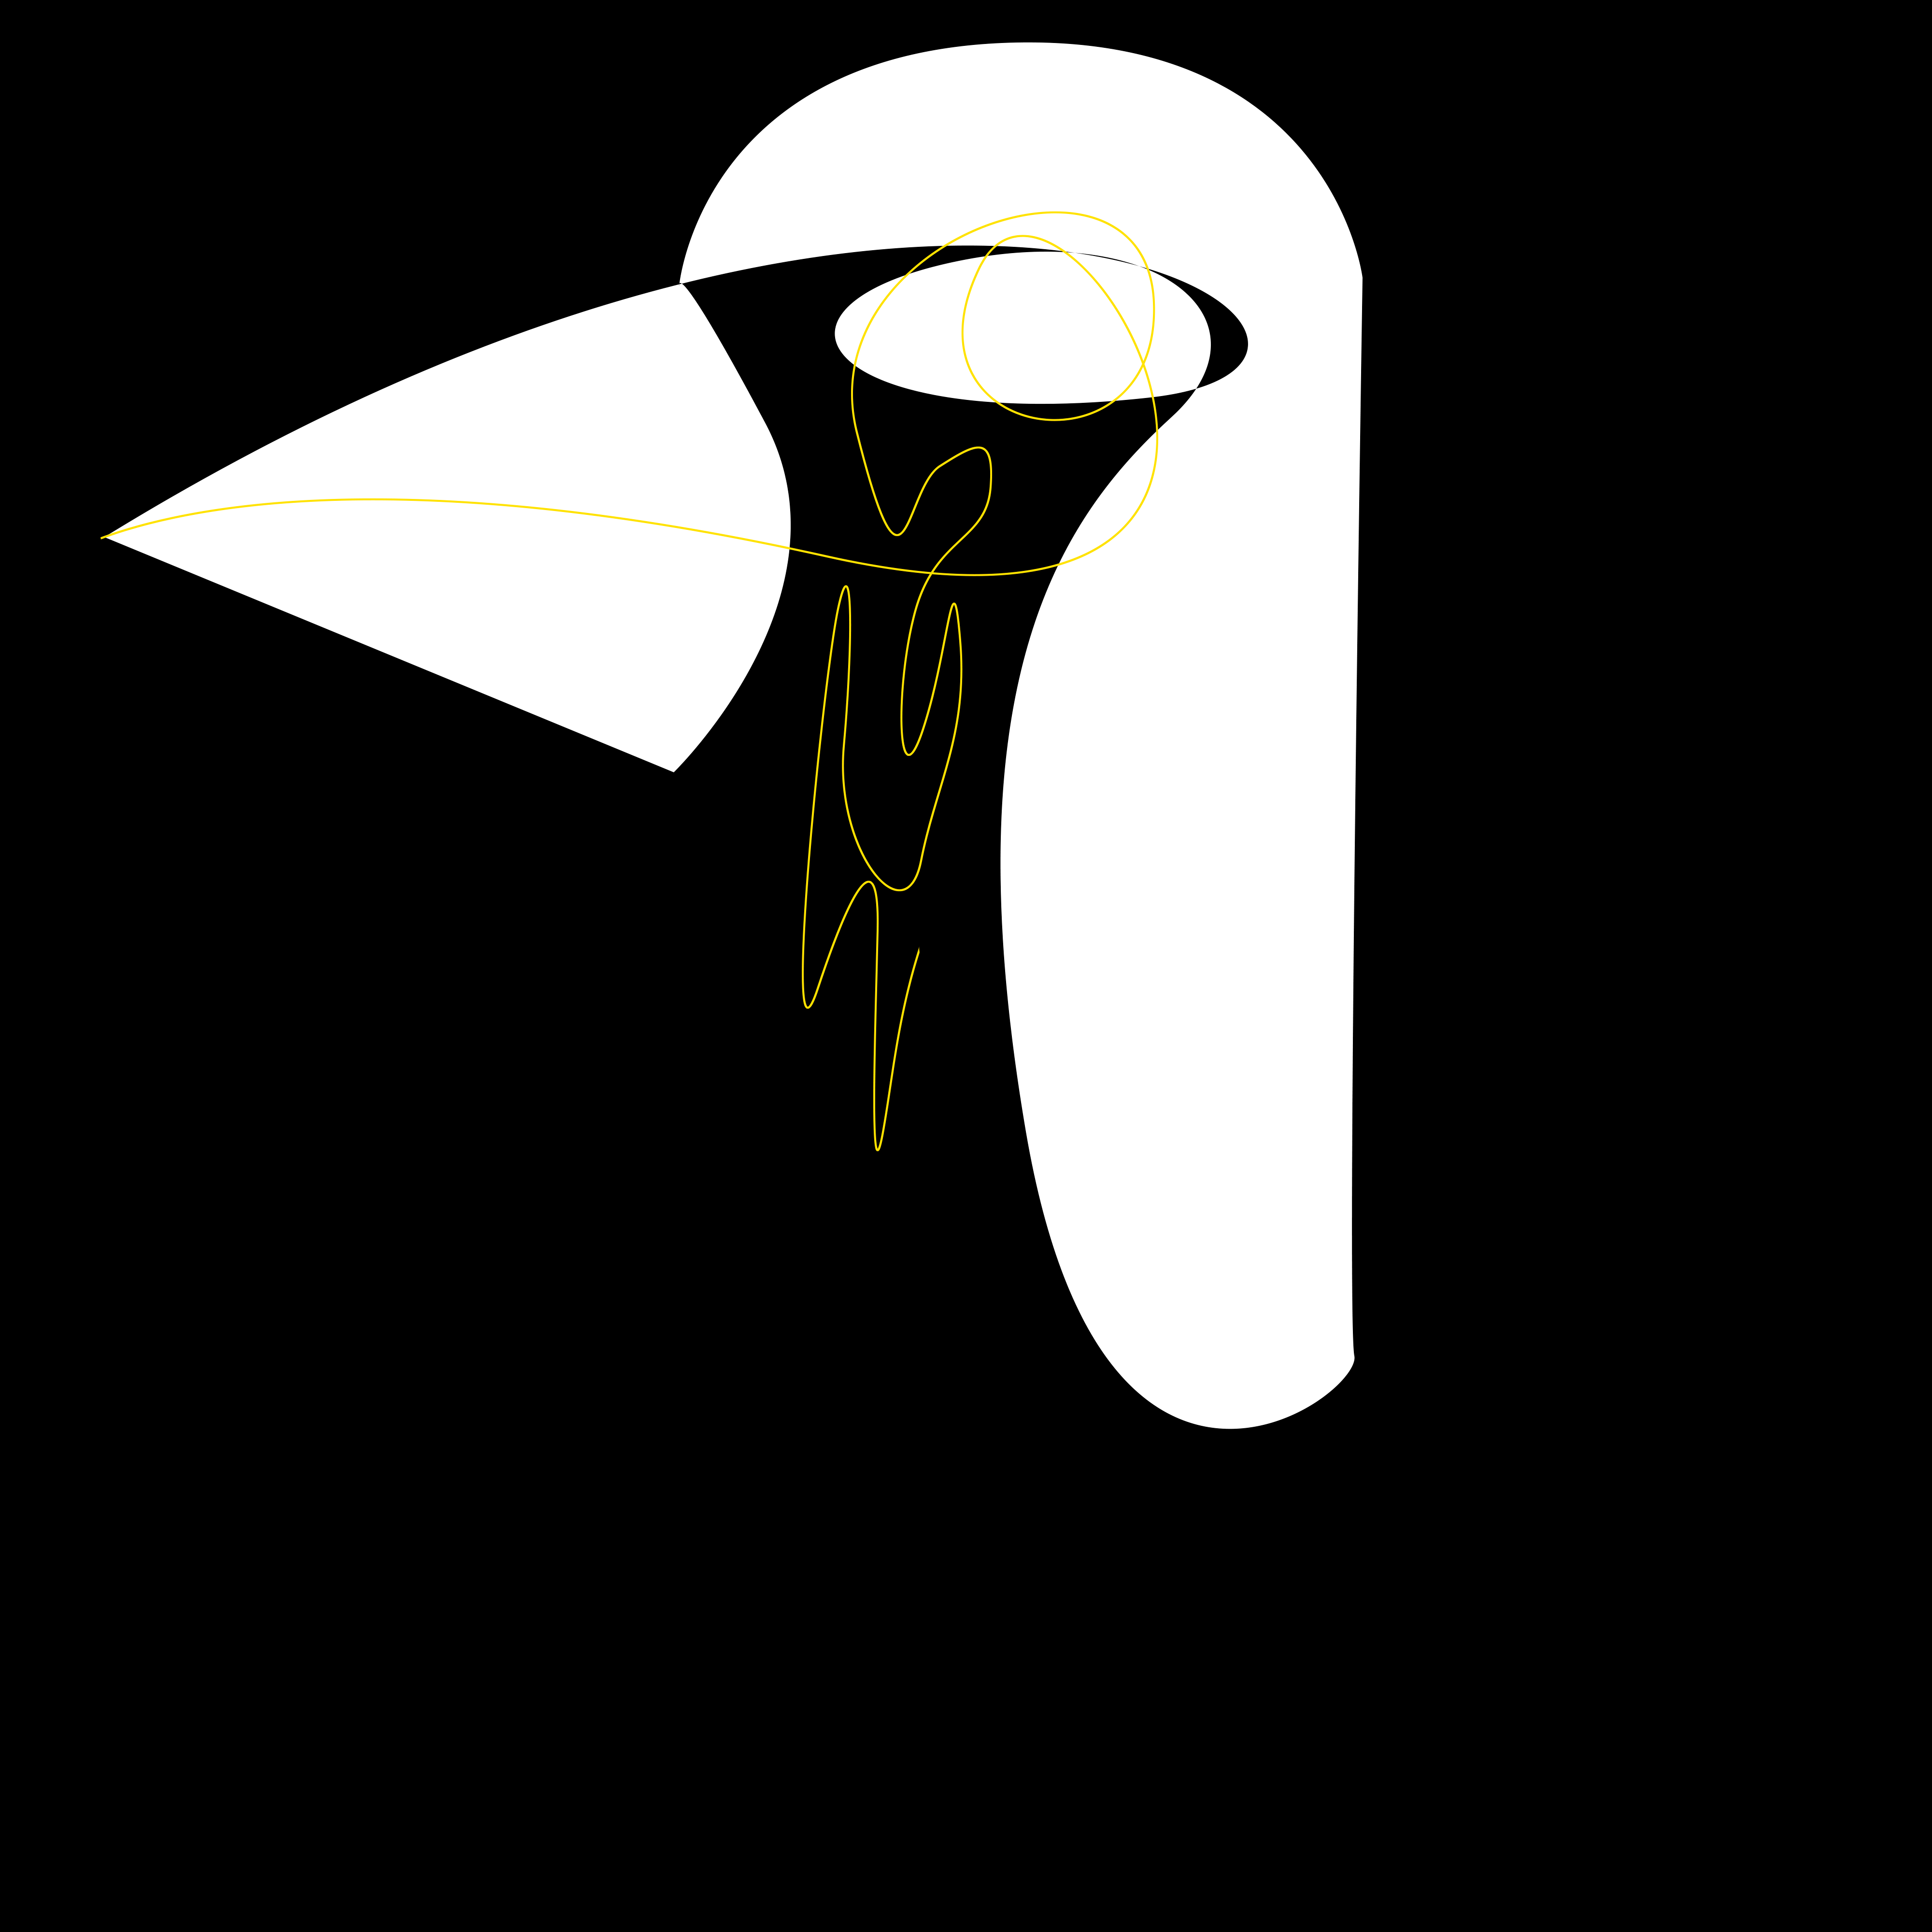
\includegraphics[scale=0.03]{Pictures/in ricordo del pinguino cameriere.png}
%\caption{Fiamme.}\label{fig:figura}
\qquad\qquad
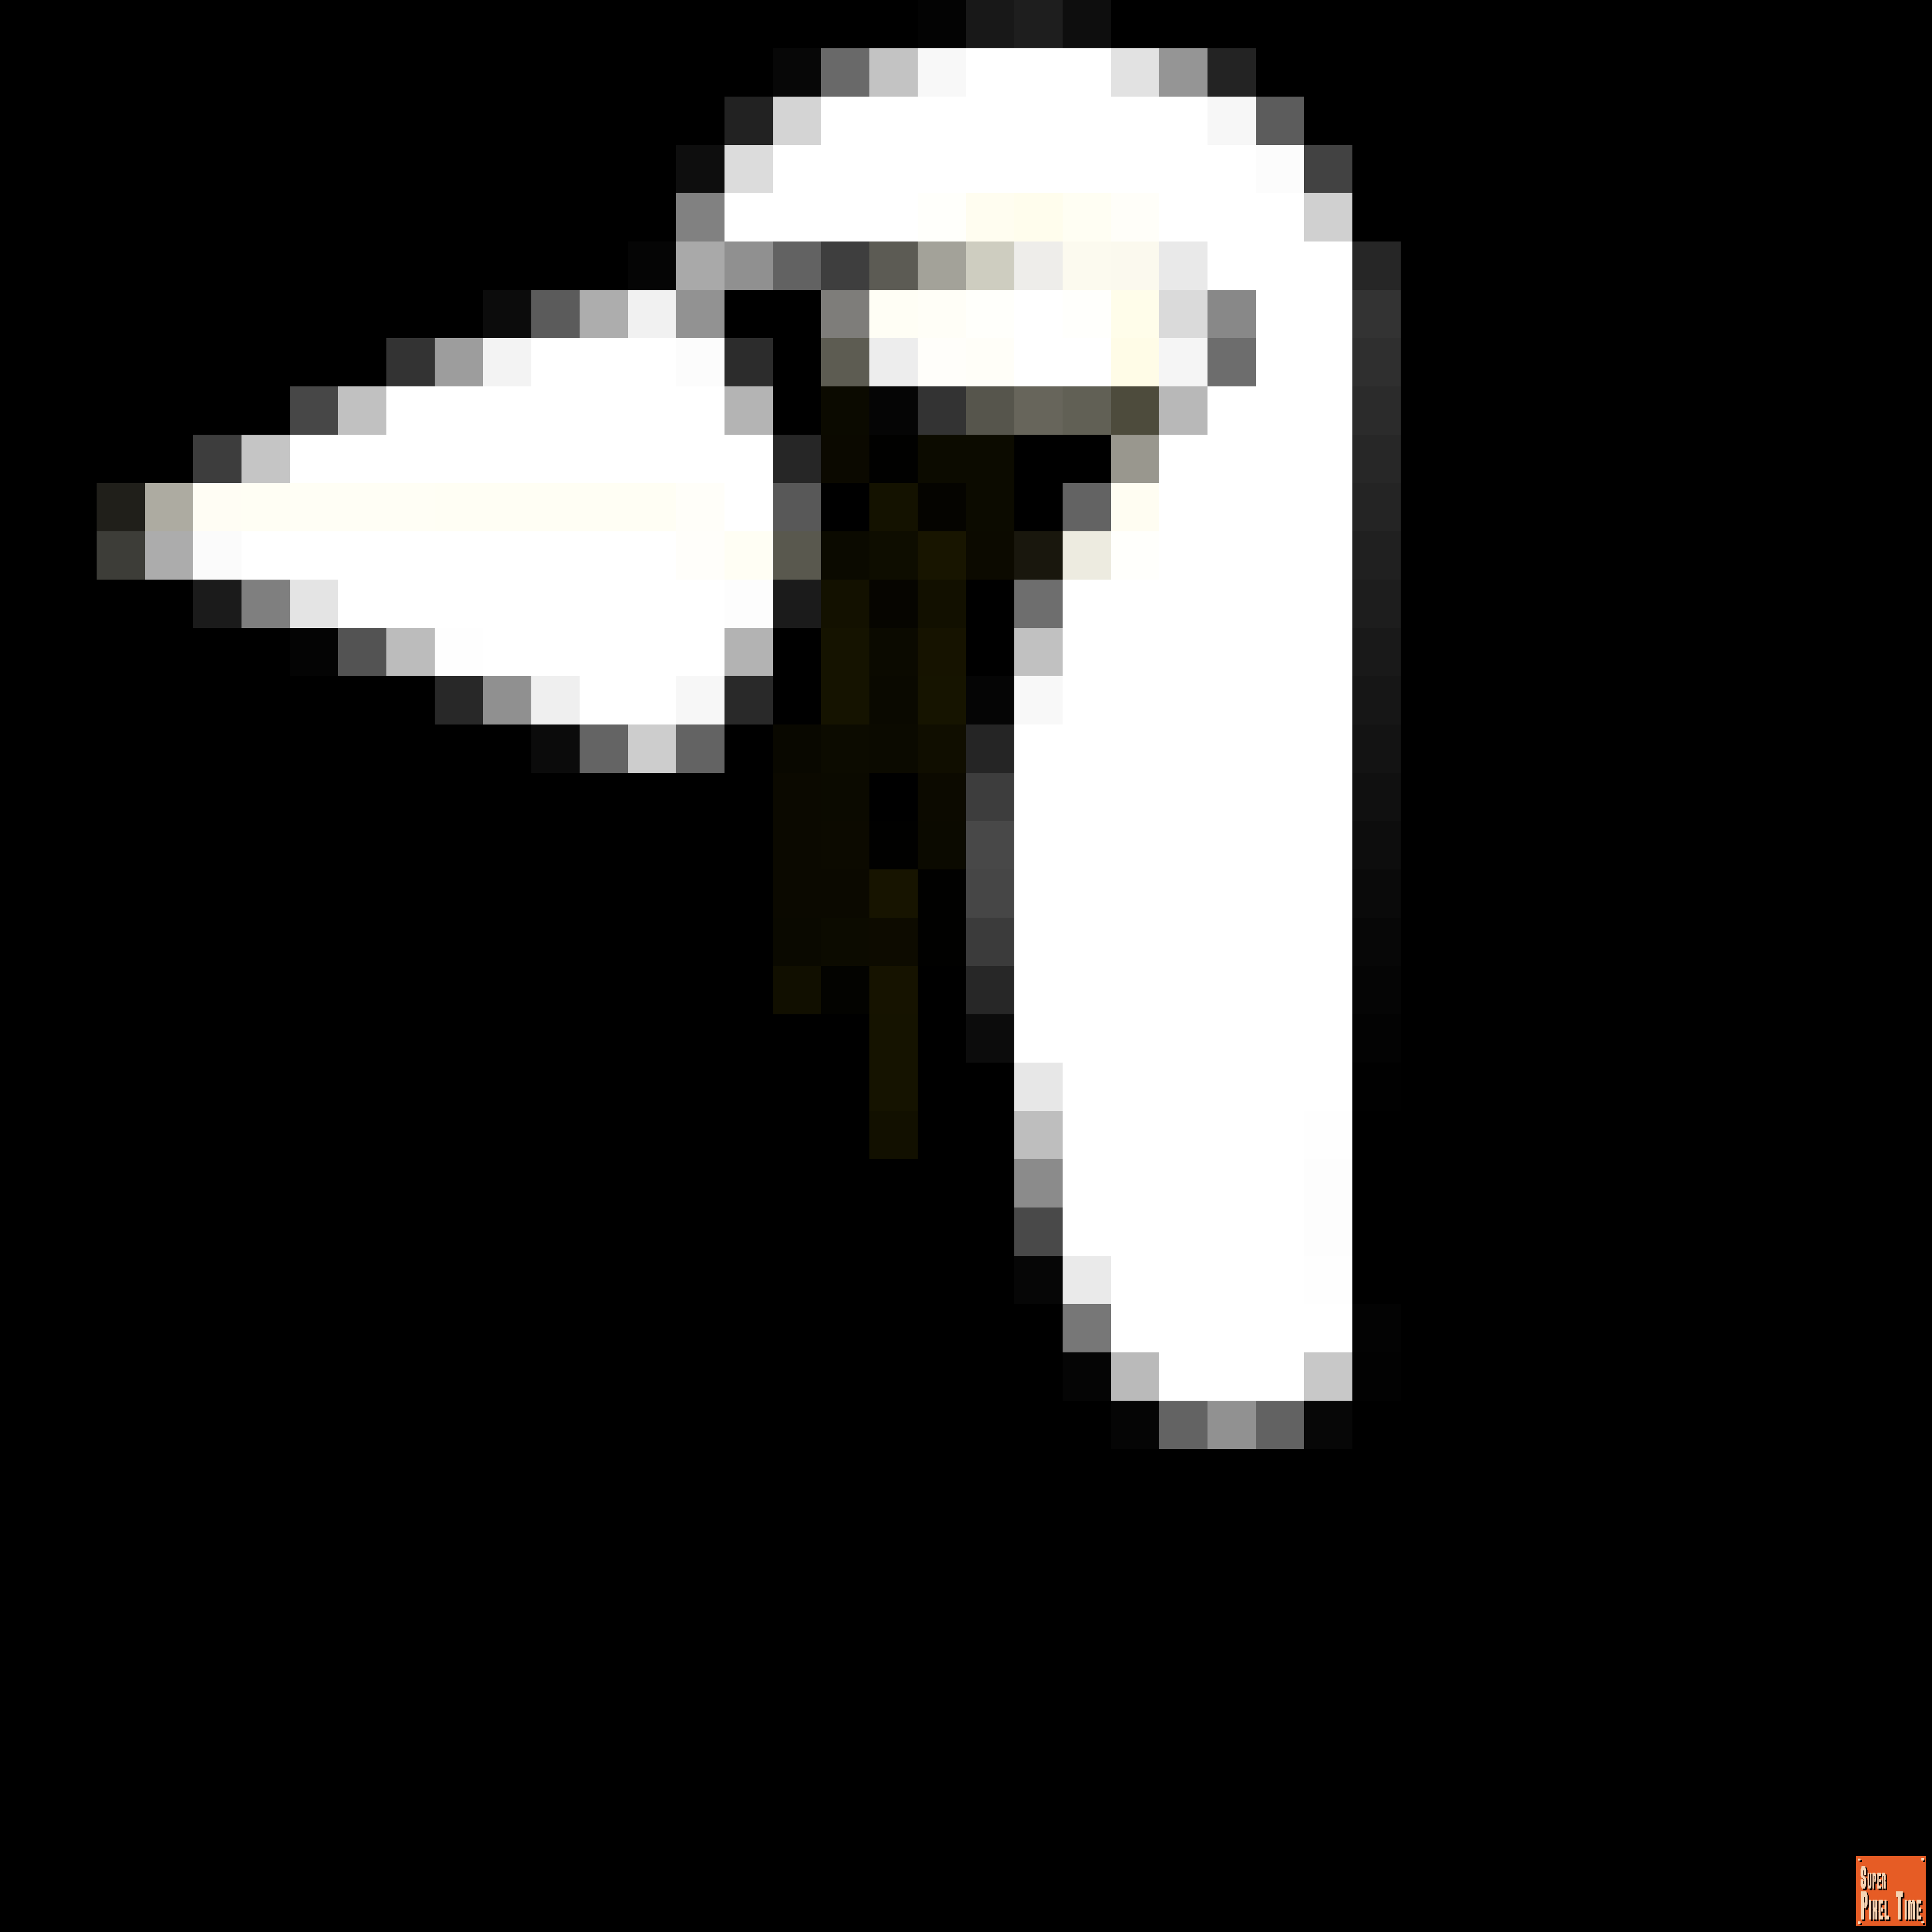
\includegraphics[scale=0.03]{Pictures/canvas80x80.png}
\caption{Confronto immagine originale e immagine codificate utilizzando una griglia 80x80.}\label{fig:figura}
\end{figure}

E' semplice vedere come ad una griglia più fitta corrisponda una miglior qualità dell'immagine, questo è il concetto di "risoluzione di un'immagine". 
Una miglior risoluzione però costa, come anticipato, in termini di memoria. Una griglia 4x4 corrisponde a 16 pixel, ad una griglia 80x80 corrispondono invece 6400 pixel! Questo vuol dire che la seconda immagine pesa 400 volte di più della prima.


Volendo definire in maniera più precisa cosa sia un'immagine digitale, diremmo che è una funzione da $\mathbb R^2$ in $\mathbb R^3$ siccome, date in input due cordinate questa funzione ci restituisce un colore (che è formato da 3 canali RGB).

\section{Cosa sono i filtri}
Una volta capito che un'immagine è una funzione possiamo definire un filtro come una seconda funzione che convoluta alla prima da il risultato richiesto.


Una equazione alle derivate parziali (PDE) esprime una evoluzione, sia u la nostra immagine e $u_0$ lo stato in cui si trova inzialmente, allora per convoluzione possiamo dire che 

\begin{equation} \label{eq:eq3}
u(x)=\frac{1}{w(x)}\int\int d(x-\xi)\Tilde{d}(u_0(x) -u_0(\xi))u_0(\xi)d\xi.
\end{equation}

\centering con  $w(x) = \int\int d(x-\xi)\Tilde{d}(u_0(x) -u_0(\xi))d\xi$\newline


\raggedright

Prendiamo in esame l'equazione del calore



\begin{equation} \label{eq:eq2}
\begin{cases}

\frac{\partial u}{\partial t}(t,x)-\Delta u(t,x) = 0 \ x \in \mathbb R^2, t\ge 0 \ .\\ 

u(0,x) = u_0(x)\ . \\

\end{cases}
\end{equation}









\bibliography{references}



\end{document}

\